Nick Vosseteig

2015-01-30

building

\begin{tabular}{|p{5cm}|p{5cm}|}
 \hline
 building&
 Added support for the robot frame and the linear slides as well as a mechanism to flip the deflector up. We also did some minor repairs to the wiring. We also added a stopper so we can pull the goals without touching the tube. It all went well, but since the linear slides are moved to the other side of the robot we will have to rewire part of it to get the encoders attached correctly.
 \\
 \hline
\end{tabular}

\section*{Building}
This week I mainly worked on adding the support to the robot. The linear slides were pretty tough to work with because they were bent out of place because of the way it was built, so I added some support to it on the top and bottom so that it stays in line. I also had to take apart the back supports so that I could add the stopper to prevent the tube from hitting the robot while pulling/pushing it. I took apart the back and then moved the supports up and added another one to keep the frame sturdy. David and Philip worked on the mechanism to flip the deflector which is a servo with a long tetrix piece attached to it. 
 The tube stopper is just a straight tetrix piece on the back of our robot that we needed to add because we moved the linear slides to the side and they acted as a stopper previously. It was tough to do because the holes on the support beams on the back of the robot didn’t line up. I ended up putting it diagonally so that it would line up and it works well after testing.	

Here is a picture of the tube stopper/pusher:
\begin{center}
 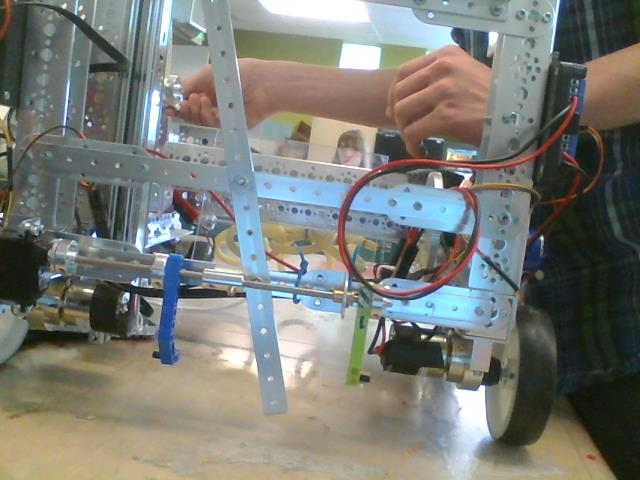
\includegraphics[width=215px]{./Entries/Images/stopper.jpg}
\end{center}